% #######################################
% ########### FILL THESE IN #############
% #######################################
\def\mytitle{THINK OF A TITLE FOR REPORT}
\def\mykeywords{C Sharp, Console, Draughts, Checkers, Command Line Interface, Marc Reid}
\def\myauthor{Marc Reid}
\def\contact{03001588@live.napier.ac.uk}
\def\mymodule{Algorithms and Data Structures (SET09117)}
% #######################################
% #### YOU DON'T NEED TO TOUCH BELOW ####
% #######################################
\documentclass[10pt, a4paper]{article}
\usepackage[a4paper,outer=1.5cm,inner=1.5cm,top=1.75cm,bottom=1.5cm]{geometry}
\twocolumn
\usepackage{graphicx}
\graphicspath{{./images/}}
%colour our links, remove weird boxes
\usepackage[colorlinks,linkcolor={black},citecolor={blue!80!black},urlcolor={blue!80!black}]{hyperref}
%Stop indentation on new paragraphs
\usepackage[parfill]{parskip}
%% Arial-like font
\IfFileExists{uarial.sty}
{
    \usepackage[english]{babel}
    \usepackage[T1]{fontenc}
    \usepackage{uarial}
    \renewcommand{\familydefault}{\sfdefault}
}{
    \GenericError{}{Couldn't find Arial font}{ you may need to install 'nonfree' fonts on your system}{}
    \usepackage{lmodern}
    \renewcommand*\familydefault{\sfdefault}
}
%Napier logo top right
\usepackage{watermark}
%Lorem Ipusm dolor please don't leave any in you final report ;)
\usepackage{lipsum}
\usepackage{xcolor}
\usepackage{listings}
%give us the Capital H that we all know and love
\usepackage{float}
%tone down the line spacing after section titles
\usepackage{titlesec}
%Cool maths printing
\usepackage{amsmath}
%PseudoCode
\usepackage{algorithm2e}

\usepackage[labelformat=empty]{caption}


\usepackage[toc,page]{appendix}


\titlespacing{\subsection}{0pt}{\parskip}{-3pt}
\titlespacing{\subsubsection}{0pt}{\parskip}{-\parskip}
\titlespacing{\paragraph}{0pt}{\parskip}{\parskip}
\newcommand{\figuremacro}[5]{
    \begin{figure}[#1]
        \centering
        \includegraphics[width=#5\columnwidth]{#2}
        \caption[#3]{\textbf{#3}#4}
        \label{fig:#2}
    \end{figure}
}

\lstset{
	escapeinside={/*@}{@*/}, language=C++,
	basicstyle=\fontsize{8.5}{12}\selectfont,
	numbers=left,numbersep=2pt,xleftmargin=2pt,frame=tb,
    columns=fullflexible,showstringspaces=false,tabsize=4,
    keepspaces=true,showtabs=false,showspaces=false,
    backgroundcolor=\color{white}, morekeywords={inline,public,
    class,private,protected,struct},captionpos=t,lineskip=-0.4em,
	aboveskip=10pt, extendedchars=true, breaklines=true,
	prebreak = \raisebox{0ex}[0ex][0ex]{\ensuremath{\hookleftarrow}},
	keywordstyle=\color[rgb]{0,0,1},
	commentstyle=\color[rgb]{0.133,0.545,0.133},
	stringstyle=\color[rgb]{0.627,0.126,0.941}
}

\thiswatermark{\centering \put(336.5,-38.0){
\includegraphics[scale=0.8]{logo}} }
\title{\mytitle}
\author{\myauthor\hspace{1em}\\\contact\\Edinburgh Napier University\hspace{0.5em}-\hspace{0.5em}\mymodule}
\date{}
\hypersetup{pdfauthor=\myauthor,pdftitle=\mytitle,pdfkeywords=\mykeywords}
\sloppy
% ###############################################################################
% ########### START FROM HERE ###################################################
% ###############################################################################
\begin{document}
	
\maketitle  
    
\begin{abstract}
%An abstract is a 100-200 word summary of your report. It provides a brief %overview of the report by stating the purpose, defining the topic, summarising %the main sections of the report, and stating the conclusion or outcomes. An %abstract is usually written when you have completed the report
\end{abstract}


\pagenumbering{arabic} 
%\textbf{Keywords -- }{\mykeywords}
    
    
    
\section{Introduction}
The purpose of this report was to document the data structures and algorithms used during the process of designing and implementing the game Checkers (with English draughts rule set) with a command line interface in C\#.
\newline
We look in depth at how and why we implemented the data structure we did as well as explaining the logic behind the algorithms that we designed to solve the problems we faced whilst implementing the game.
\newline
There are 3 games modes included in this application:

\begin{itemize}
	\item Human vs Human
	\item Human vs A.I.
	\item A.I. vs A.I.
\end{itemize}

All game modes use the scoreboard implemented so that the players can observe the number of normal pieces and king pieces that are still present on the board for both players. The session score is also displayed in the scoreboard so that the players can play multiple games and determine the winner at the end of the current session.

Whilst there is a human player, they will have access to the features Undo and Redo. It was decided that during an A.I. vs A.I. these features would not be necessary. All game modes have access to the Replay feature as it was considered convenient to be able to replay full games regardless of whether a human player was involved in the game or not.
\newline
The A.I. vs A.I. game mode is the only game mode which imposes a draw as an end game condition. This was implemented to stop A.I. vs A.I. from becoming excessive in length due to the A.I.'s movement being random.

 
    
\section{Design}   
During this project a test-driven development approach was used in conjunction with an agile methodology. This is where the code is developed incrementally in sprints with the project only moving on to the next sprint once the testing of the work done, has been passed. We will look at the following 3 main areas which demonstrate the primary design choices that were made during development.
    
        
    \subsection{Interface}
    The application runs from the command line as this is what was asked for in the coursework specification with the proviso that we could develop the application with a graphical interface at a later date.
    
    
    	\subsubsection{CLI Playing Board}
    	To represent the board visually in the CLI, characters from the Windows character map application were used to create a custom design. The priority when designing the CLI board, was to ensure that it was easy to understand with good spacing to stop the screen from becoming cluttered.
    
    
     
    
    \subsection{Data Structures Used}
    We highlight the essential data structures used and explain why we used these specific data structures in the circumstances in which we did. The data structures used have assisted us in provide the features included in the application such as undo/redo and replay.     
     
    
   		\subsubsection{2-Dimensional Array}   
   		As the board for English draughts is an 8 x 8 chequered board, a 2 dimensional array[8,8] named \textit{positionsArray} is used to represent the board and store the current locations of the playing pieces. Each player starts with 12 normal pieces which are stored in \textit{positionsArray} as the strings 'X' and 'O'. To represent the kings, the strings stored are '|X|' and '|O|', the player can only acquire a king when they reach the opposite end of the board with a normal piece.
   		The array is updated after every turn is made, then all the contents of each index in \textit{positionsArray}, are concatenated together separated by a comma into a single string with the last value either a 'X' or an 'O' to indicate who has just taken their turn. Every time the string is created it then gets popped on to a stack called \textit{undoStack} and enqueued in to a queue called \textit{replayQueue}.
   
    
    
  		\subsubsection{Queue}
  		The queue data structure was selected for the replay feature as it uses the First-In-First-Out method for storing and retrieving information. This meant that we could add (enqueue) the string comprised of the current playing piece positions to the back of the queue after every turn. When the user selects to replay the current match, the application enters a loop which will iterate through all the string stored in the queue. A pause has been added to the loop, so that the replay can be followed by the human eye.
   
      
  		\subsubsection{Stack}
		The stack data structure is used to aid the implementation of both the undo and redo features. A stack uses the Last-In-Last-Out method for storing and retrieving information, which meant we could synergise the stacks together, to provide effective undo and redo features.
  		\newline
  		Both the queue and stack data structures selected offer improved performance over the other data structures available which could perform similar tasks but would be slower, such as an array or a list.
  
      
  		\subsubsection{List}
  		The list data structure is used twice in the application, both times it has been used as the number of values it could store at any one time will vary from move to move. It was decided that as the size of the data structure needed could not accurately be predicted a list would be the best option as it adjusts its size as needed. This removes the potential for an out of range exception when accessing the data structure selected.
    
    
    
 	\subsection{Algorithms Used}
 	The application has many algorithms which when all combined help to produce a robust version of the game Checkers. We will look at the algorithms that are essential for the application to simulate multiple games.
    
    	\subsubsection{Valid Move Check}
    	If a player has no valid moves available, then they lose the game. To enforce this rule, we used a valid move check algorithm. The valid move check takes place before the user has entered the Y and X co-ordinates of the piece they wish to move. The method \textit{AreThereAnyValidMoves()} is called (from the Player class) which returns a Boolean value depending on whether the current player has any available move to play or not.
    	\newline
    	The algorithm starts by:  
    	
   
   		\begin{itemize}
	   		\item Looping through the textit{positionsArray} checking every index for a string that matches the current players normal piece or a king piece.  
	   		\item Once a piece is found, the algorithm then checks if that piece can capture an opponent's piece.
	   		\item If not, then the algorithm checks if the piece can complete a successful move. 
			\item If after all the current players pieces have been checked and neither the capture or move checks return true, then the current player loses the game as there are no available moves to be made. 
   		\end{itemize}
   
   
    
    
    	\subsubsection{Force Capture} 
    	In the English draughts rule set if there is a capture available the player must make that move, unless there are multiple captures where the player can choose which capture to make. After the player has entered the Y and X co-ordinates of the piece they want to move and the tile they want to move the piece to, the method \textit{ForcedCaptureCheck()} is called (from the Player class).
    	\newline
    	This algorithm starts in the same way as the valid move check algorithm does by:    
    
    	\begin{itemize}
	   		\item Looping through the \textit{positionsArray} checking every index for a string that matches the current players normal piece or a king piece.
	    	\item When a piece is found, the algorithm checks if that piece can capture an opponent's piece.
	    	\item If that piece can capture an opponent's piece, the algorithm takes the Y and X co-ordinates and concatenates them together storing the value in a list called \textit{listOfForcedMoves}.
	    	\item Once the algorithm has looped through all the array, storing all the potential moves the current player can make.
	    	\item The algorithm takes the Y and X co-ordinates that the player entered as the values for the piece they want to move, concatenates them together then compares that value with the values stored on the list \textit{listOfForcedMoves}.
	    	\item If the co-ordinates entered match any of the values stored on the list, then that is an allowed move.
	    	\item The algorithm passes the co-ordinates to the method \textit{PlayerMove()} which allows the move to continue.
	    	\item If the co-ordinates entered do not match any of the values stored on the list, then the move the player wants to make is not allowed.
	    	\item A message informs the player that they must play the capture move available to them.
    	\end{itemize} 
    
    
    	\subsubsection{A.I.}    	
    
    	In this application we have included the ability to play against an A.I. player or to watch A.I. vs A.I. games. The A.I. implemented, is from our own design and as this is the first version of the A.I. we have concentrated on making sure the logic is sound and that the A.I. class integrates well with the application to provide a good platform from which to improve the A.I. in the future.
    	
    	The A.I. algorithm can be found in the method \textit{GetMove()} in the A.I. class. The algorithm works by first:  	
    	
    	
    	\begin{itemize}
    		\item Checking which player's turn it currently is then adding one to that players counter.    		
    		\item Then calculating the modulus of that counter and if the value equals 0 then the application will enter the path of the algorithm which searches for the current player's pieces starting from the back of the board, ending at the front. 
    		\item If the value of the modulus calculation does not equal 0 then the application will enter the path of the algorithm which searches for the current player's pieces in the opposite direction from the previous path.
    		\item For both paths, the algorithm will loop through \textit{positionsArray} looking for a king piece which can capture an opponent's piece. If one is found that move will be made and if there are no kings which can make a capture the algorithm will move on. 
    		\item The algorithm repeats the previous step except this time it searches for a normal piece which can capture an opponent's piece. If the search conditions are not met, the algorithm moves on to the next step.
    		\item Where the algorithm loops through \textit{positionsArray} searching for a king piece that has at least one move available from the four potential directions. If the king only has one move the algorithm will make that move, however if there are two or more moves available for that king the algorithm will selected at random which move to make. If there are no available moves, the algorithm will move on to the next step.
    		\item The algorithm loops through \textit{positionsArray} seeking a normal piece, once it finds one the algorithm checks if the normal piece can move in either of its potential directions. If it can the algorithm will make that move.
    		\item The algorithm will always find a move to play as before every move there is a valid move check which must return true for the application to continue to this part of the A.I. code.    		
    	\end{itemize}
    	
    	
    	
    	
    	
    	
    
    	\subsubsection{Win / Draw Conditions}
    	For a game to end, certain conditions must be met which result in either one of the players winning the match or a draw between the two A.I. players. This application has two algorithms which handle potential game ending, checks. The first algorithm checks every turn if a player has won the game.
    	\newline
    	The algorithm does this by:
    	
    	\begin{itemize}
    	\item Calling the method \textit{IsThereAWinner()} from the TheBoard class.
    	\item The method adds the value for each players kings and normal pieces together, then checks if the total equals 0.
    	\item If either player is left with 0 playing pieces, then they have lost the game.
    	\item The winning screen is shown indicating which player has won.
    	\end{itemize}
    
    	The second algorithm has only been implemented in the A.I. vs A.I. game mode. It checks every turn if the game is a draw.
    	\newline
    	This algorithm works by:
    	
    	\begin{itemize}
    	\item Calling the method \textit{IsItADraw()} from the AI class.
    	\item This method checks if the variable \textit{howManyMovesWithoutACapture} is equal to 20.
    	\item The variable \textit{howManyMovesWithoutACapture} acts as a counter and increases by 1 every time either player makes a move but not a capture.
    	\item The counter is reset to 0 every time there is a capture by either player.
    	\item This means that if both A.I. players go a combined amount of 20 turns without a capture, the game is considered a draw.
    	\end{itemize}
    	
    
    
    
    
    
    
    

    
    
    
\section{Enhancements}
During the implementation phase of this project, these were the features that were considered but either deemed to be too time intensive to implement and test before the submission date or a simplified version was implemented. These features may be implemented or improved as part of the software's evolution in the future.


    \subsection{Export and Import full game replays}
    The ability to export and import game replays, to and from a file format such as comma-separated values (.CSV).     
    The application would convert the strings that are currently used to store the positions of all the playing pieces each turn, into the Portable Draughts Notation which is the standardised notation for recording a game of checkers. 
    
       
    \subsection{Multiple rules sets available}
    Allowing the users to select which game rules they would like to play for the current session. Examples of different rule sets that could of been implemented:
     
    
    	\subsubsection{International Checkers}
    	The size of the board would have to be increased for International Checkers as the standard board size is 10 x 10 with 20 playing pieces per player. The 'flying kings' rule and the ability for 'normal' pieces to capture opponent pieces by jumping backwards would both require alterations to the movement and capturing logic.    
    	As it is a rule that the move which captures the highest number of opponent pieces must always be taken, a form of scoring system would need to be introduced to ensure that only the highest scoring move is taken by the player or AI.
    	
    
    	\subsubsection{Brazilian / Italian Checkers}
   		Both of these rule sets are only slight modifications from either English draughts or International checkers. Brazilian checkers uses the same rule set as International checkers, but these games are played on a 8 x 8 board whereas Italian checkers while played on the same size of board with a similar rule set to English draughts, there is the additional rule that 'normal' pieces cannot capture king pieces.
   		
    
    	\subsubsection{Suicide Checkers}
    	Suicide checkers, which is also known as Losing draughts, is a variation of checkers where the objective of the game is to lose all the pieces that belong to yourself before your opponent can lose all their pieces. The winner being the first player left with 0 checkers or no available moves to make. 
    	
    	
    \subsection{Improved AI}
    
   The current A.I. could be improved by implementing an algorithm which would search for each available move assigning them all a score, based on set criteria. The algorithm would then select and play the move with the highest score.    
   The current A.I. only searches either one or two tiles away diagonally before making an available move. Increasing the search distance to 3 or 4 tiles from the selected piece would survey a larger portion of the board each move and would allow a score based algorithm to adapt sooner to the opponents moves.
   
    
    
    
    
    
    
    
    
    
    
    
    
  
    
\section{Critical Evaluation}
Describe the features that I felt worked well or poorly and why I thought this.

% game is fit for purpose / follows rules/ stability from testing results

% ai vs ai game mode works well, varied results which means not the same winner all the time



    
\section{Personal Evaluation}  
Reflecting on what I learnt, the challenges I faced, the methods I used to overcome these challenges and how I feel that I performed.

%started the project earlier

%breaking the task into smaller parts and implementing them one at time and thourghly testing good plan

%no experiance from making a game in cli

%only used stack and queue in classroom exercises never in a working evnviroment

% started in wpf then converted to console. wish i'd taken the advice 

% how to use git and sourcetree

% how to use LaTeX

   
%\section{References}
%Links.....

\appendix
\newpage
\onecolumn
\section{Appendix A}

\begin{figure}[H]
	\centering	
	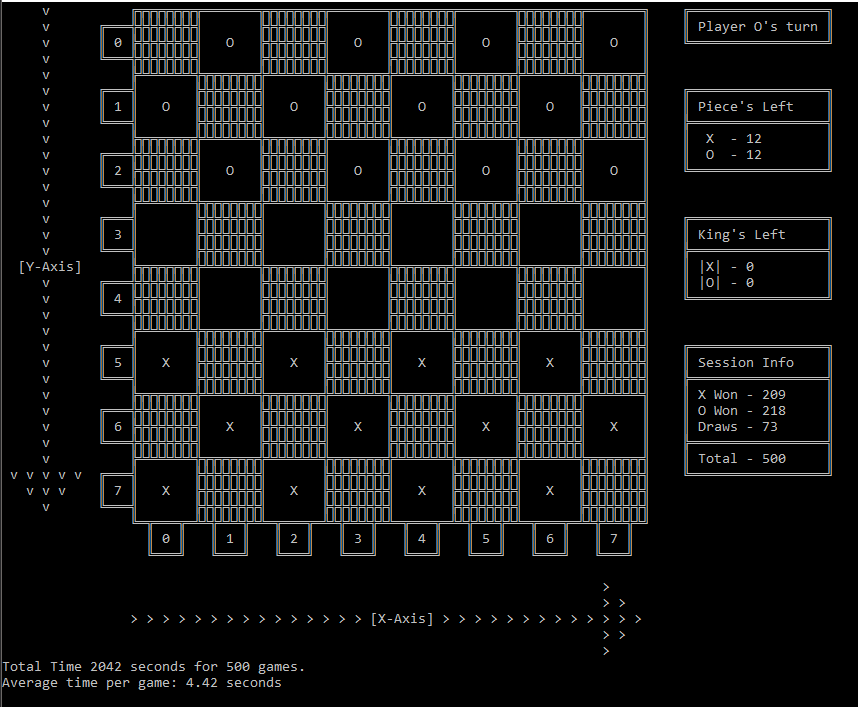
\includegraphics[scale=0.8]{RunOne500}
	\caption{Run 01 - 500 A.I. vs A.I. played}		
\end{figure}


\newpage
\section{Appendix B}

\begin{figure}[H]
	\centering
	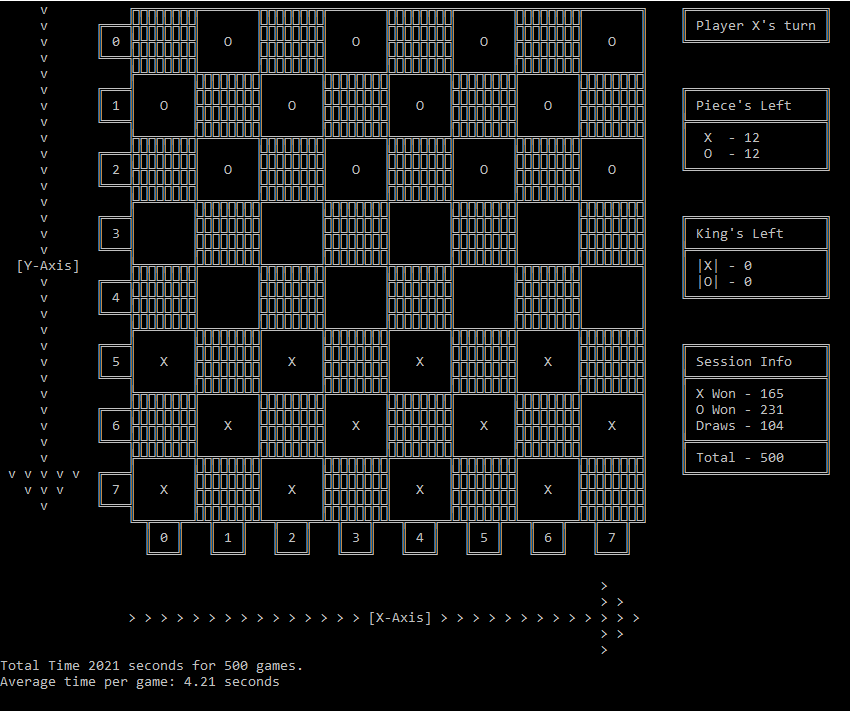
\includegraphics[scale=0.8]{RunTwo500}
	\caption{Run 02 - 500 A.I. vs A.I. played}
\end{figure}


\section{Appendix C}

\begin{figure}[H]
	\centering	
	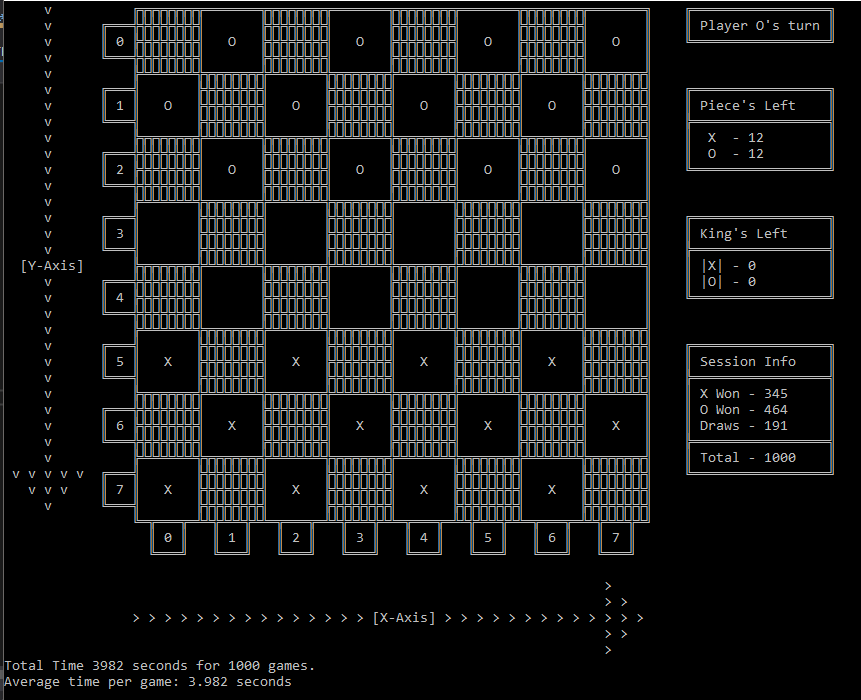
\includegraphics[scale=0.8]{RunOne1000}
	\caption{Run 01 - 1000 A.I. vs A.I. played}		
\end{figure}


\newpage
\section{Appendix D}

\begin{figure}[H]
	\centering
	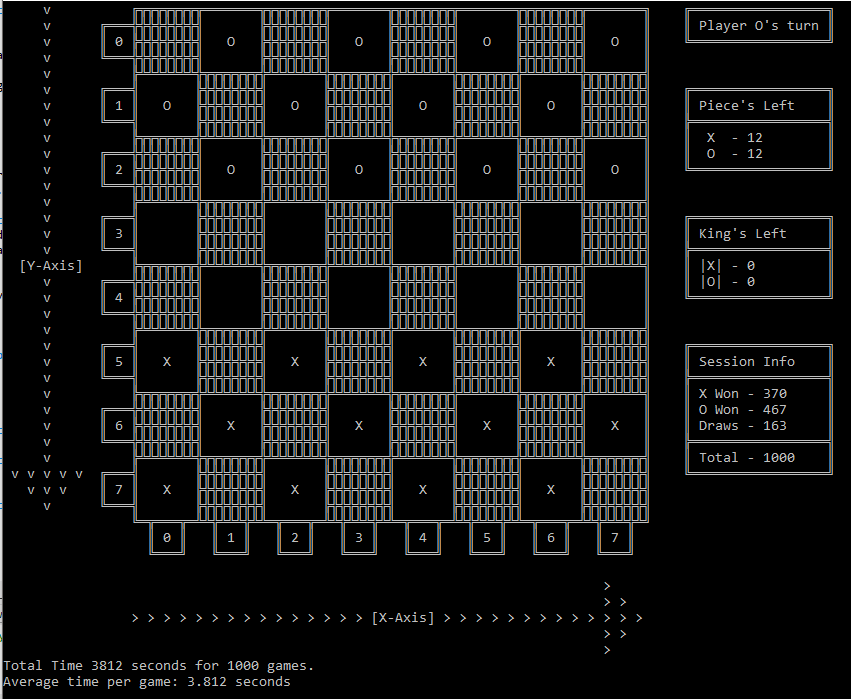
\includegraphics[scale=0.8]{RunTwo1000}
	\caption{Run 02 - 1000 A.I. vs A.I. played}
\end{figure}


\section{Appendix E}

\begin{figure}[H]
	\centering	
	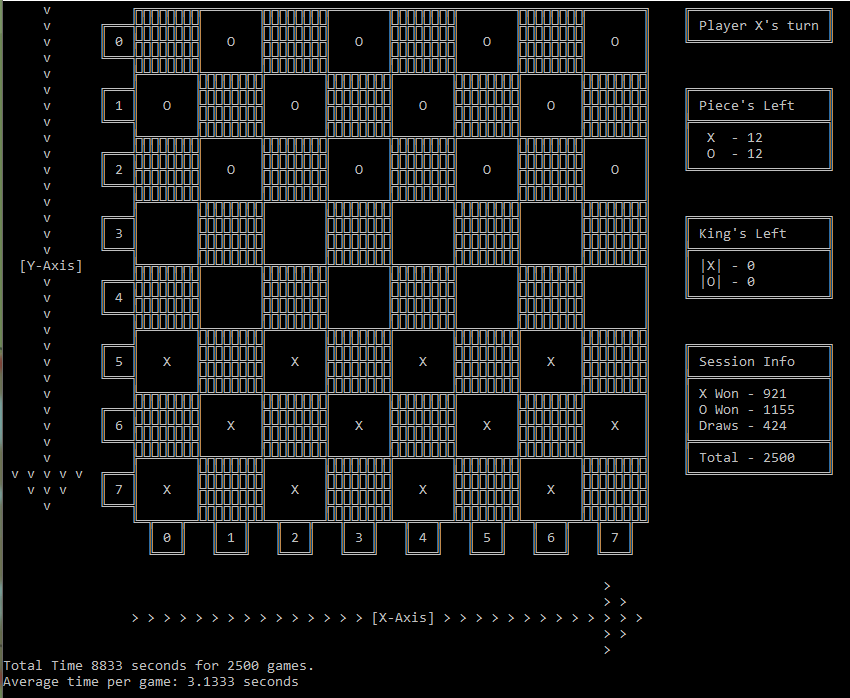
\includegraphics[scale=0.8]{RunOne2500}
	\caption{Run 01 - 2500 A.I. vs A.I. played}		
\end{figure}


\newpage
\section{Appendix F}

\begin{figure}[H]
	\centering
	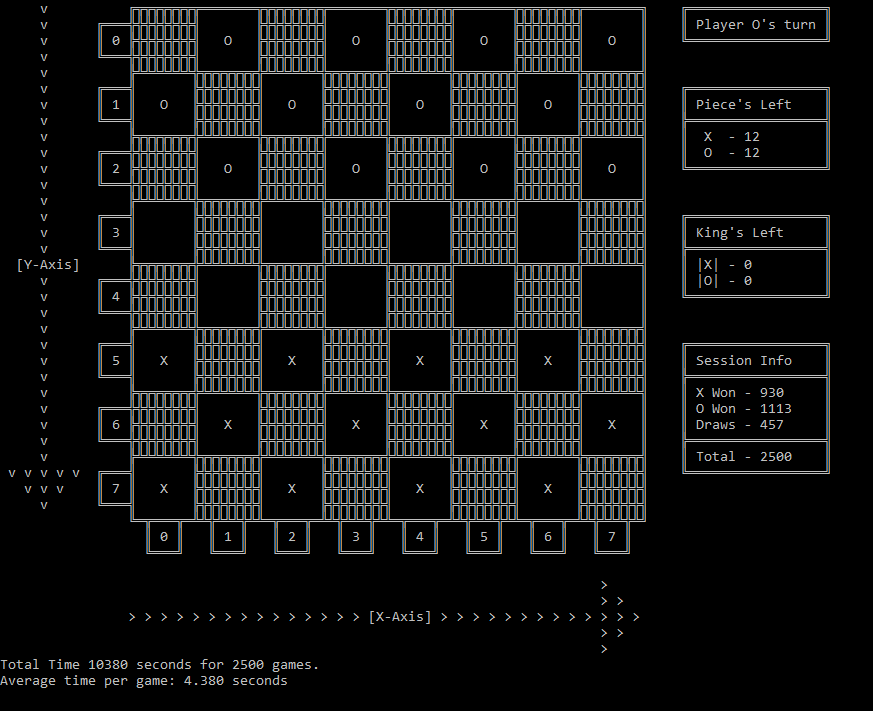
\includegraphics[scale=0.8]{RunTwo2500}
	\caption{Run 02 - 2500 A.I. vs A.I. played}
\end{figure}   

\end{document}